\par\clearpage
\section{Anhang: Frontend-Bilder}

\graphicspath{{Frontend/assets/}{Abgabe_4/Frontend/assets/}}

Die folgenden Abbildungen zeigen zentrale Ansichten des Frontends. Sie dokumentieren sowohl die tabellarischen Übersichtsseiten als auch die erweiterten Patientenaktionen.

\subsection{Übersichtsseiten}

\begin{figure}[H]
    \centering
    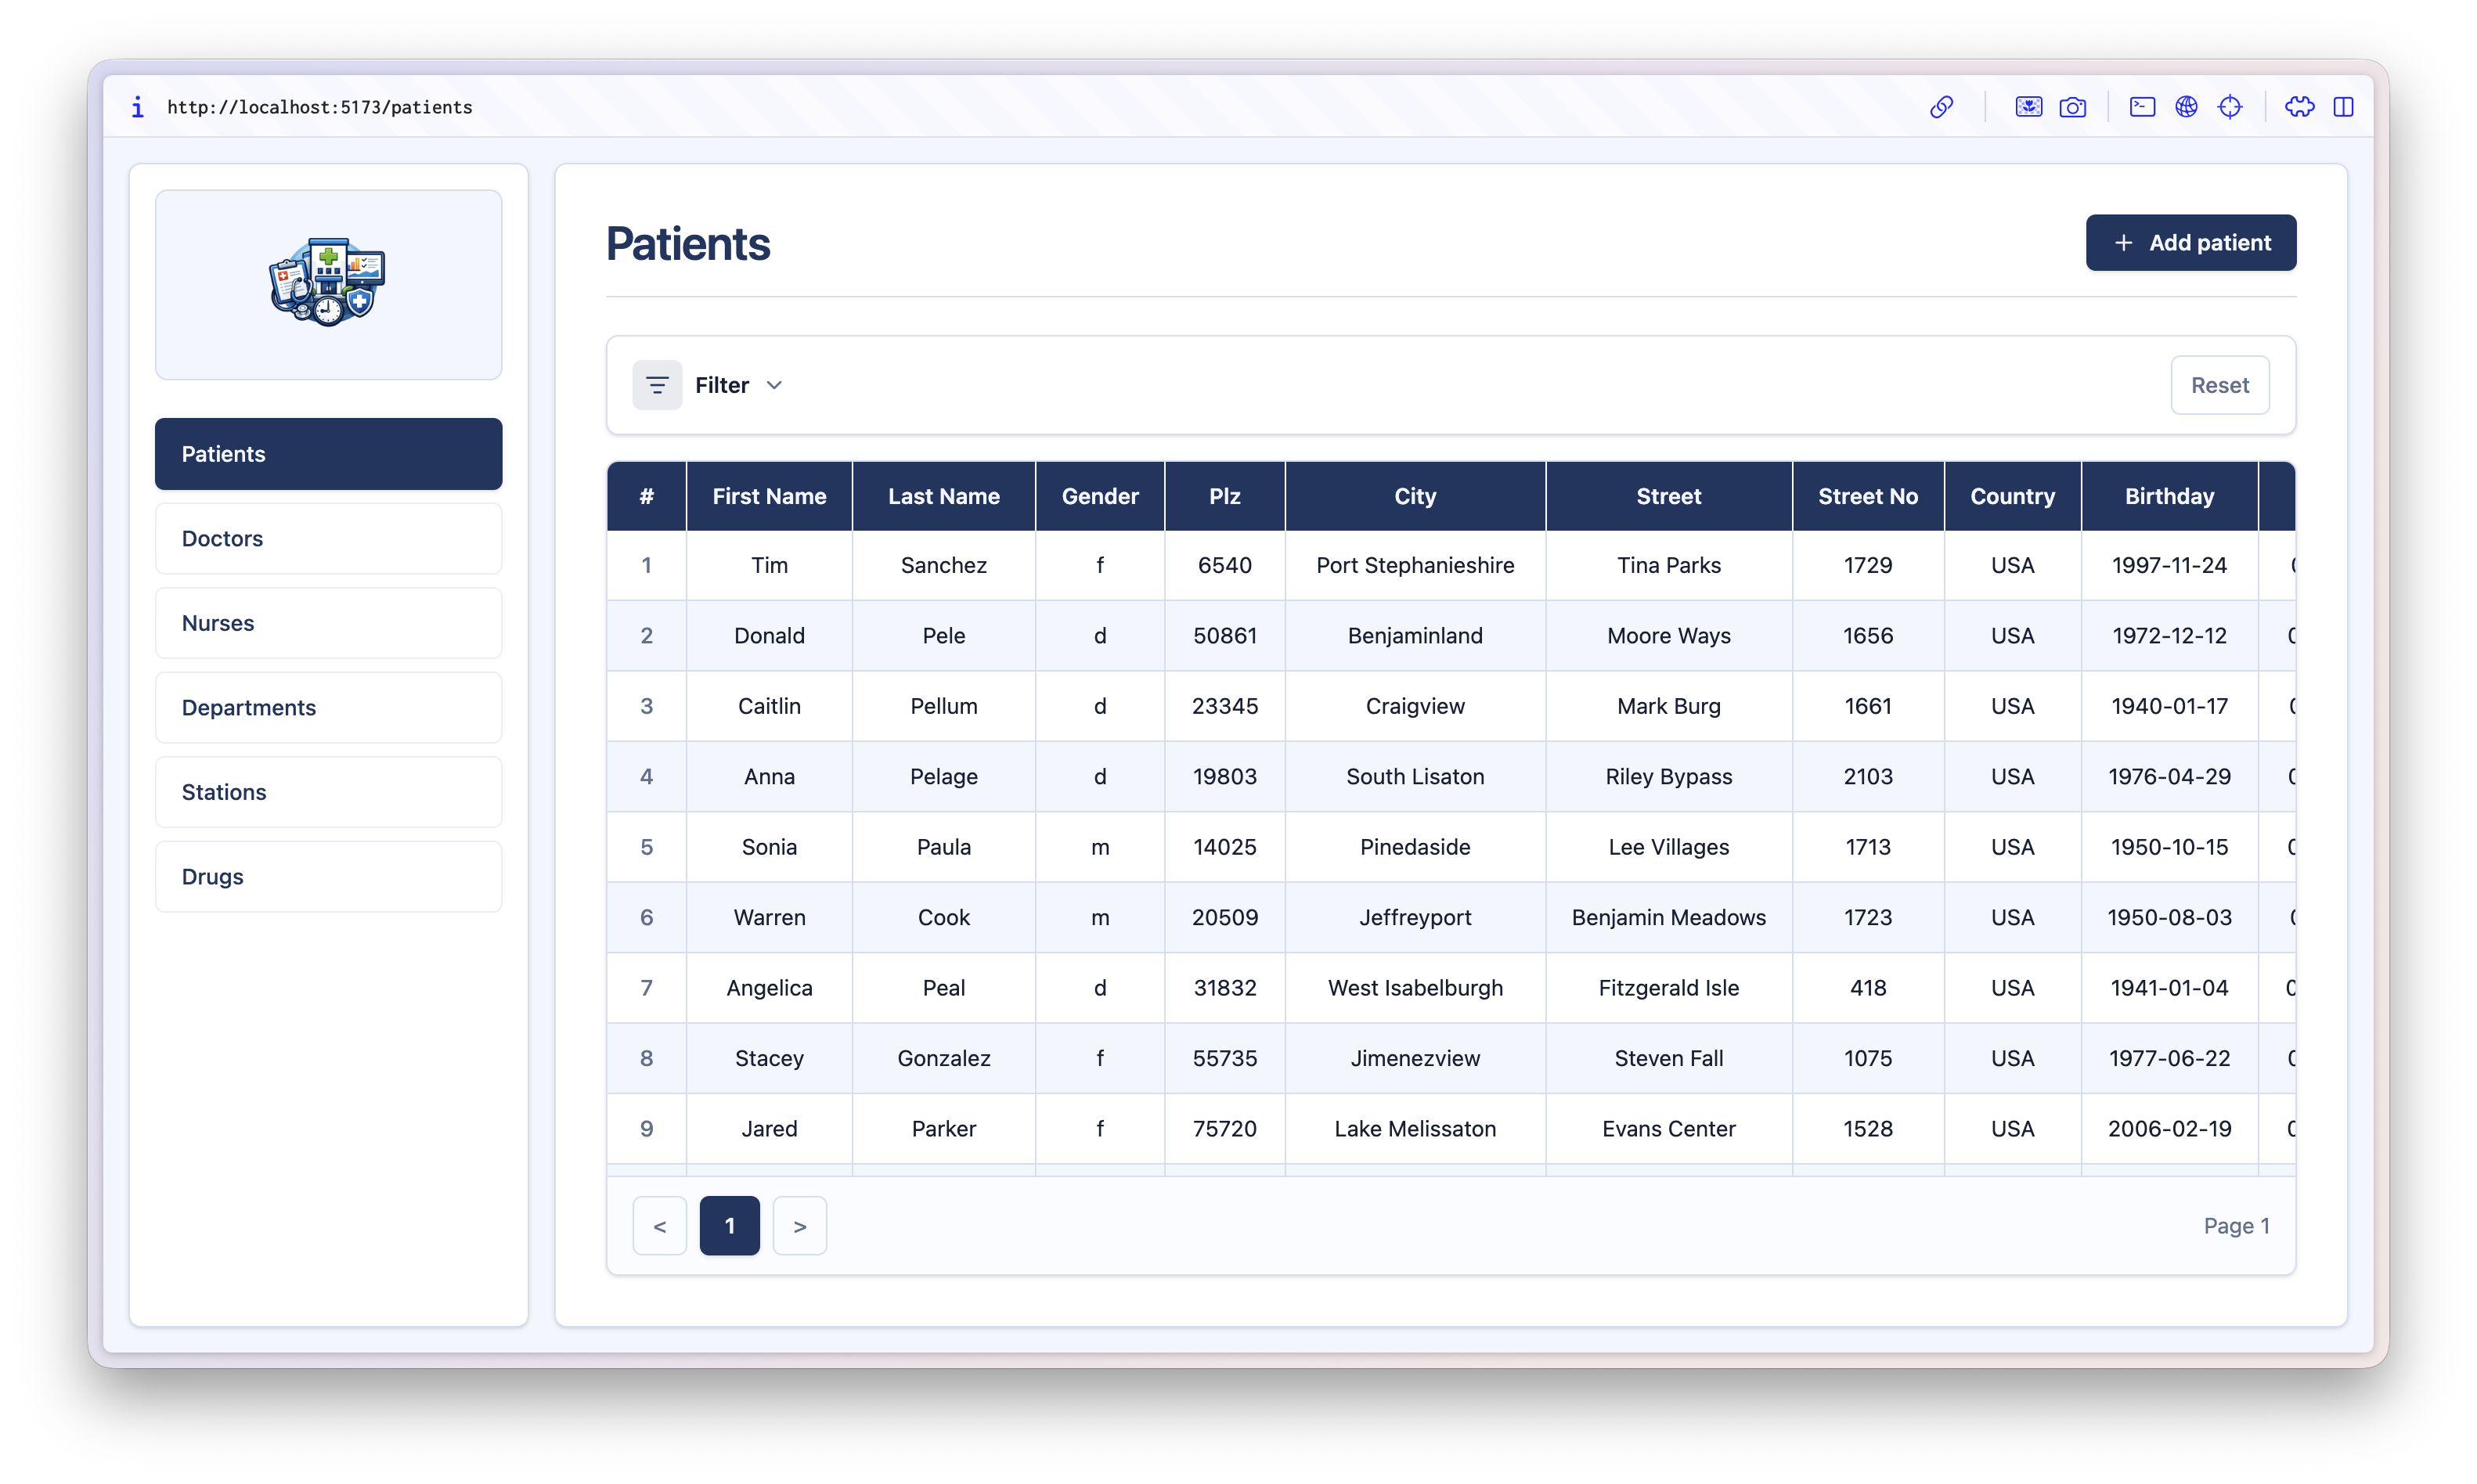
\includegraphics[width=\textwidth,height=0.78\textheight,keepaspectratio]{patients.png}
    \caption{Patientenübersicht mit Tabellenansicht}
    \label{fig:frontend-patients}
\end{figure}

\begin{figure}[H]
    \centering
    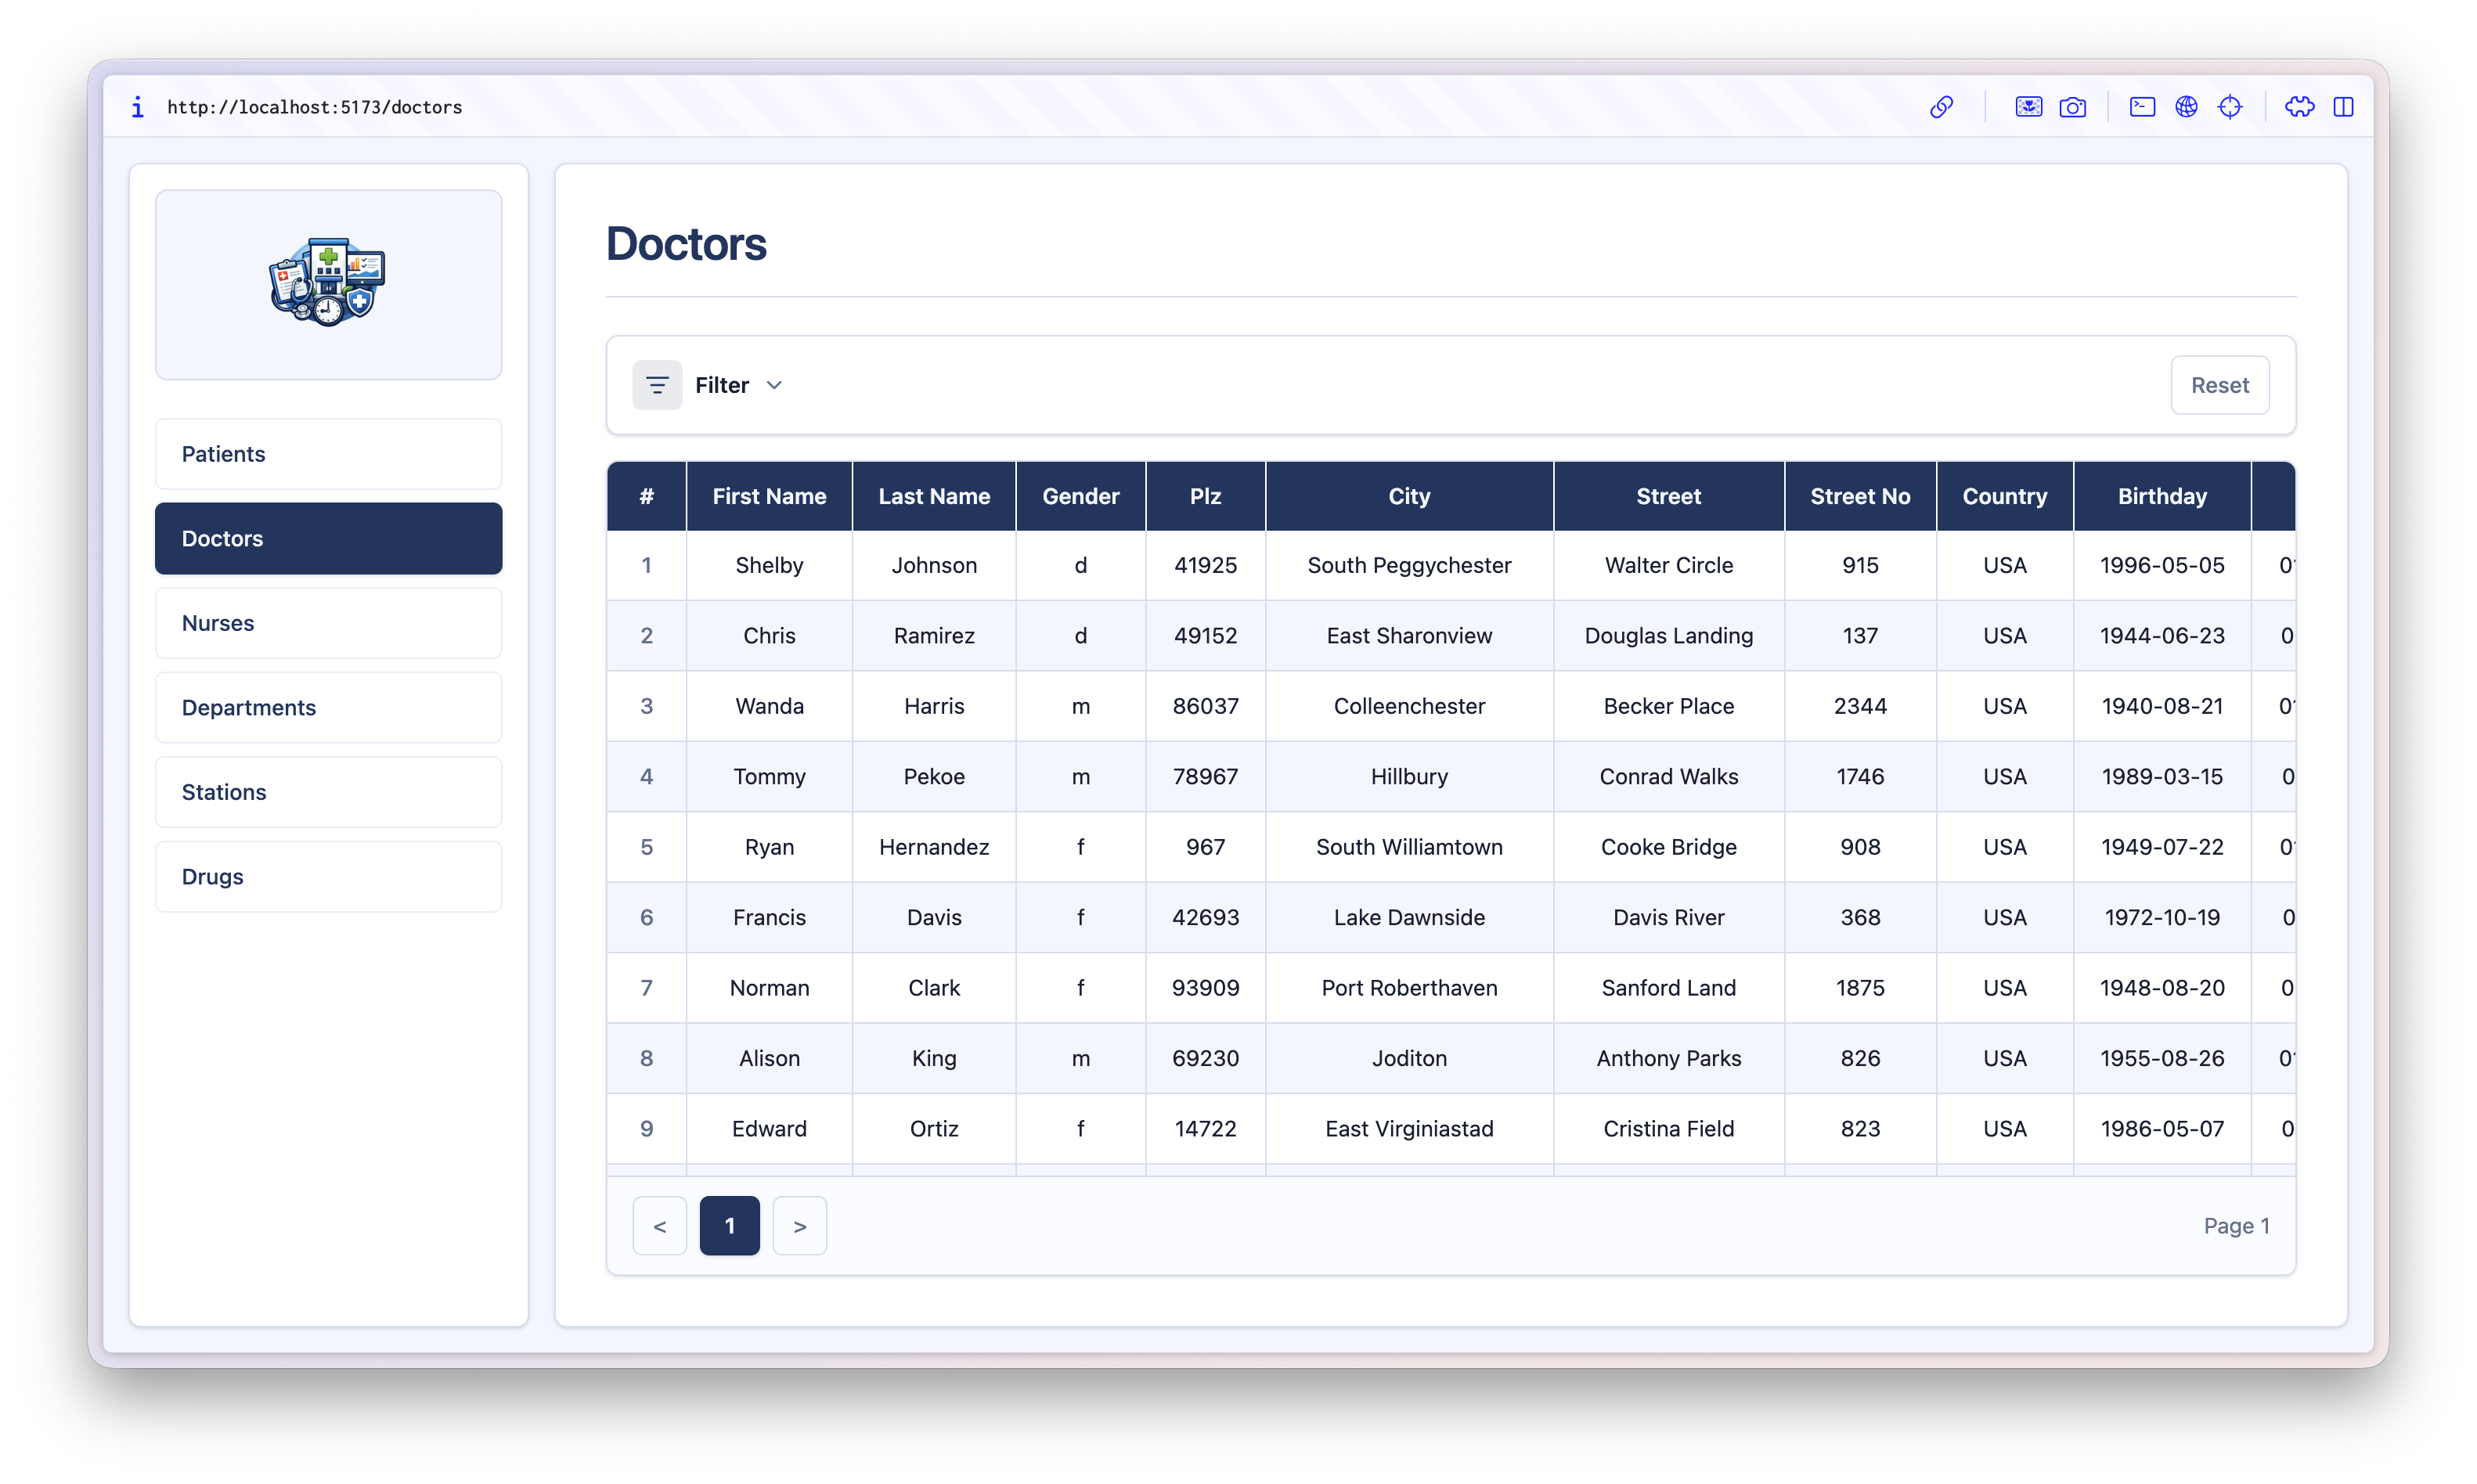
\includegraphics[width=\textwidth,height=0.78\textheight,keepaspectratio]{doctors.png}
    \caption{Ärzteübersicht mit Filter- und Tabellenstruktur}
    \label{fig:frontend-doctors}
\end{figure}

\begin{figure}[H]
    \centering
    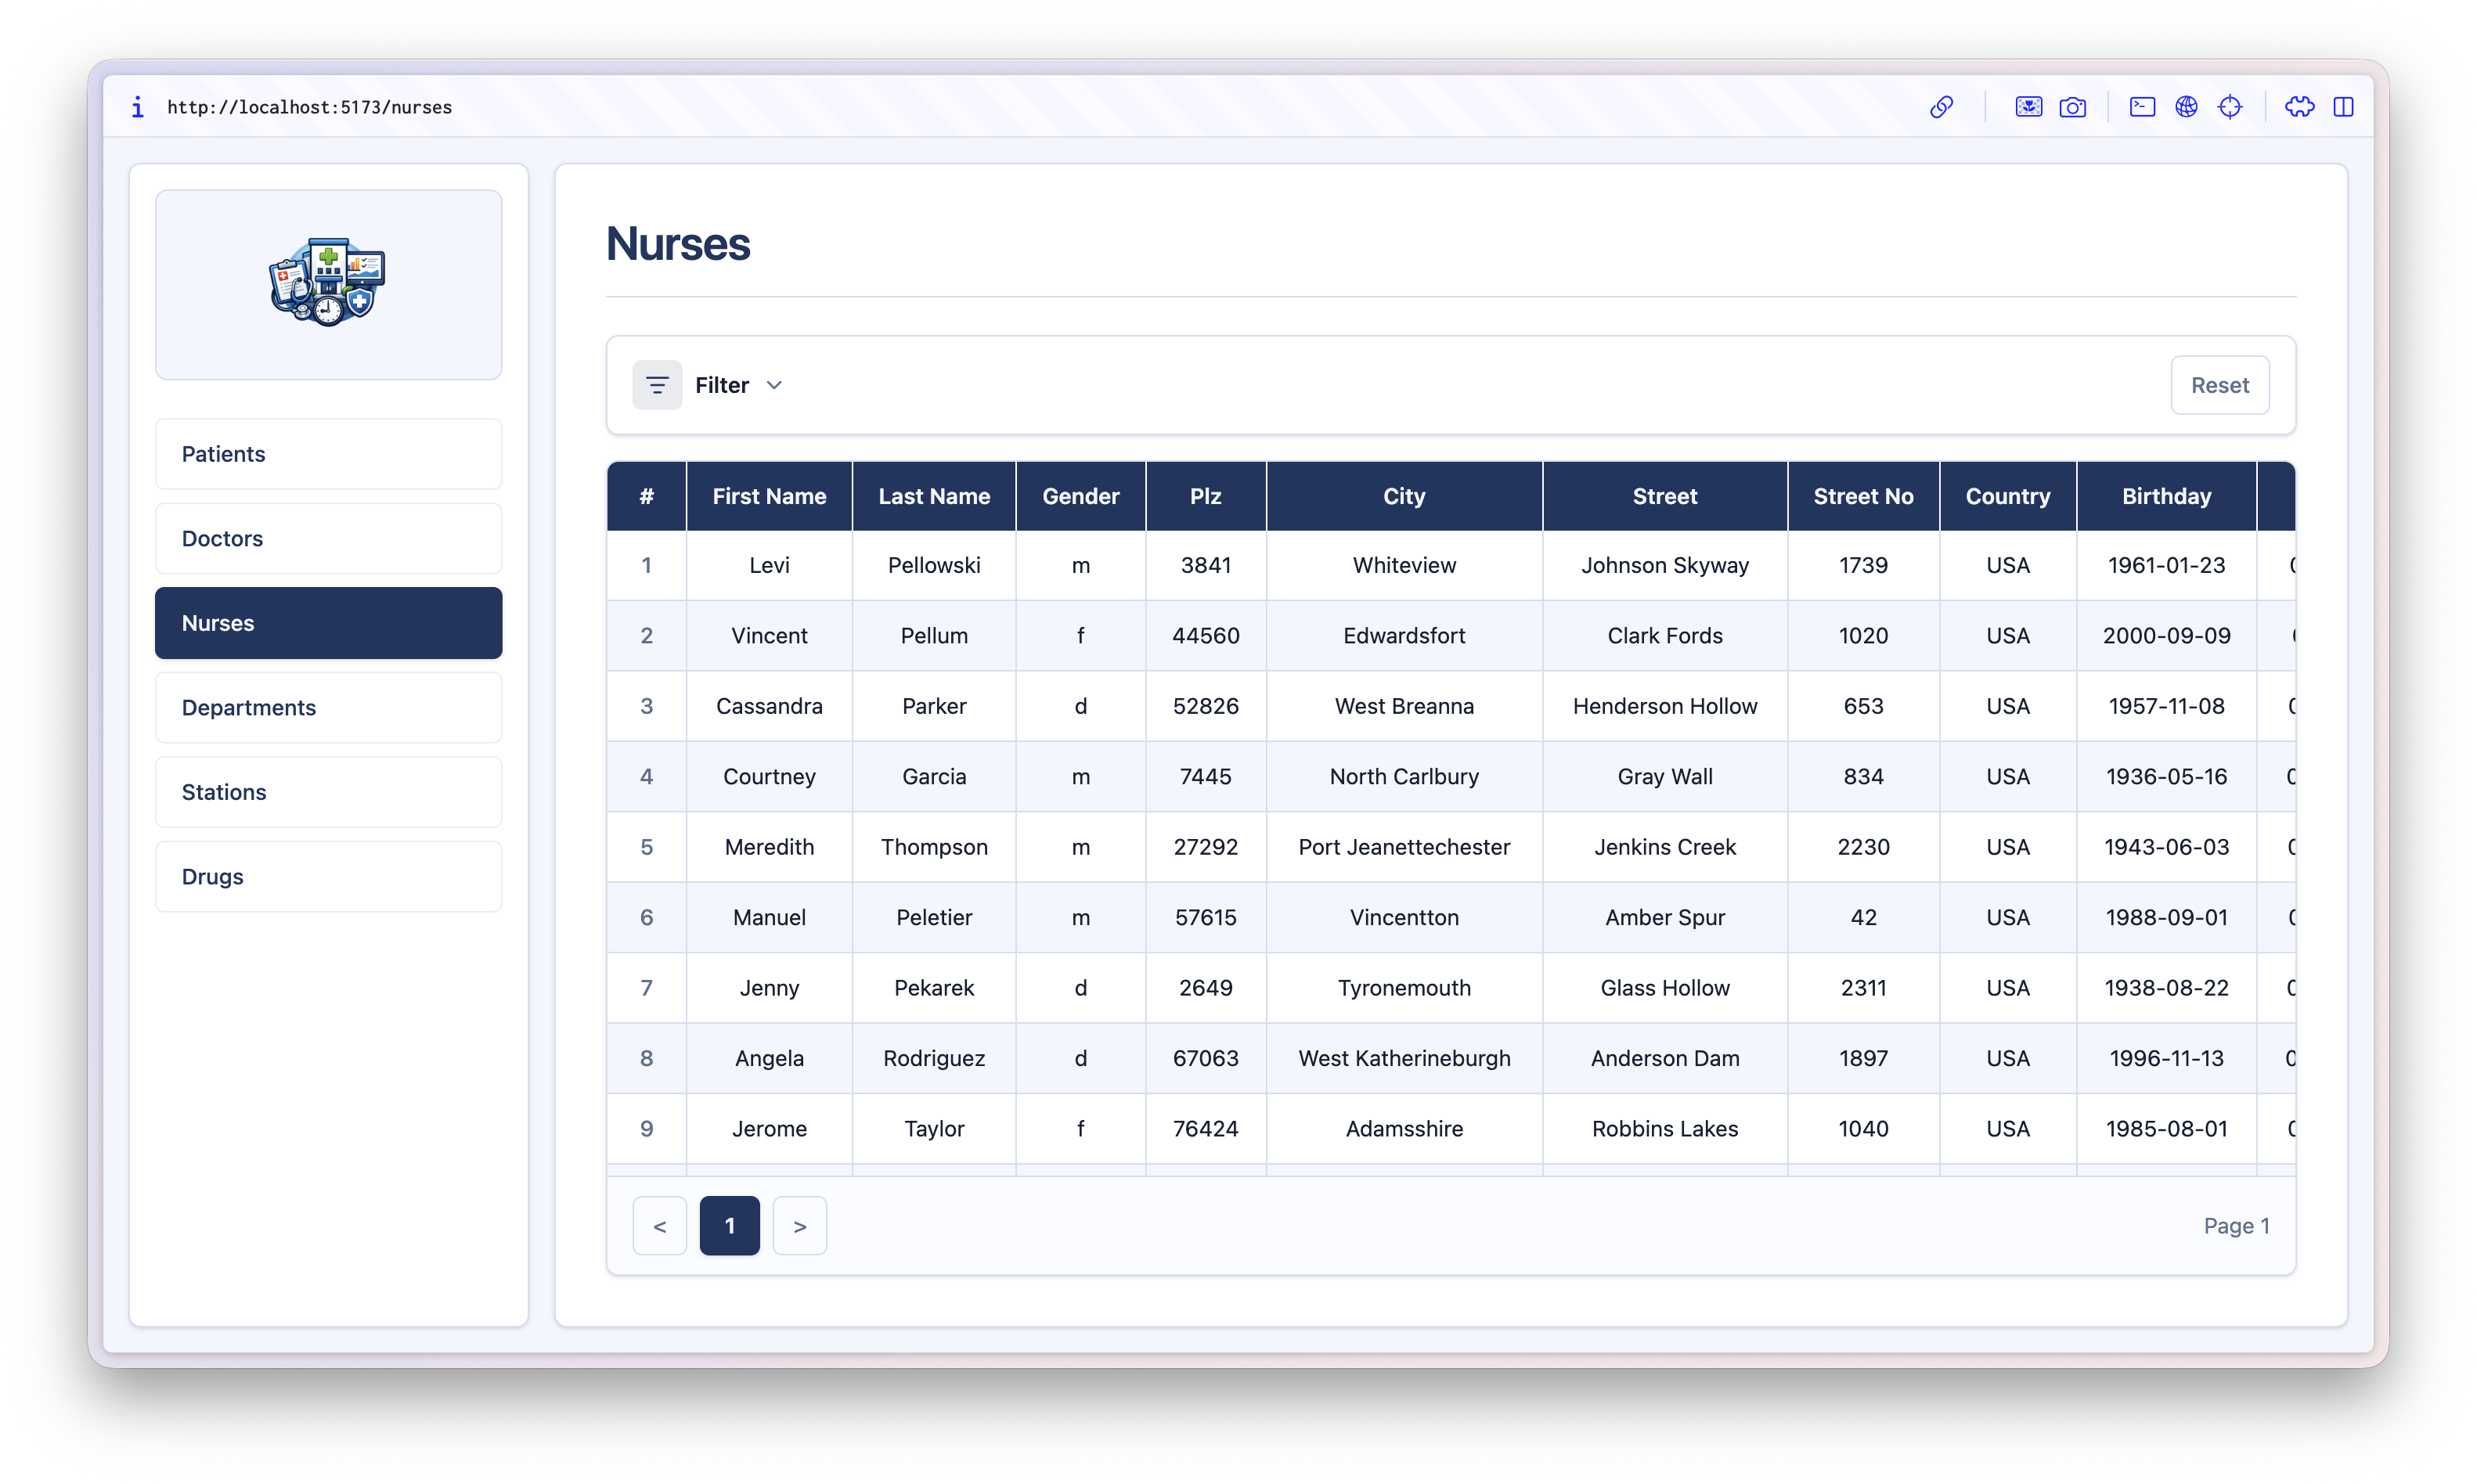
\includegraphics[width=\textwidth,height=0.78\textheight,keepaspectratio]{nurses.png}
    \caption{Pflegekräfteübersicht}
    \label{fig:frontend-nurses}
\end{figure}

\begin{figure}[H]
    \centering
    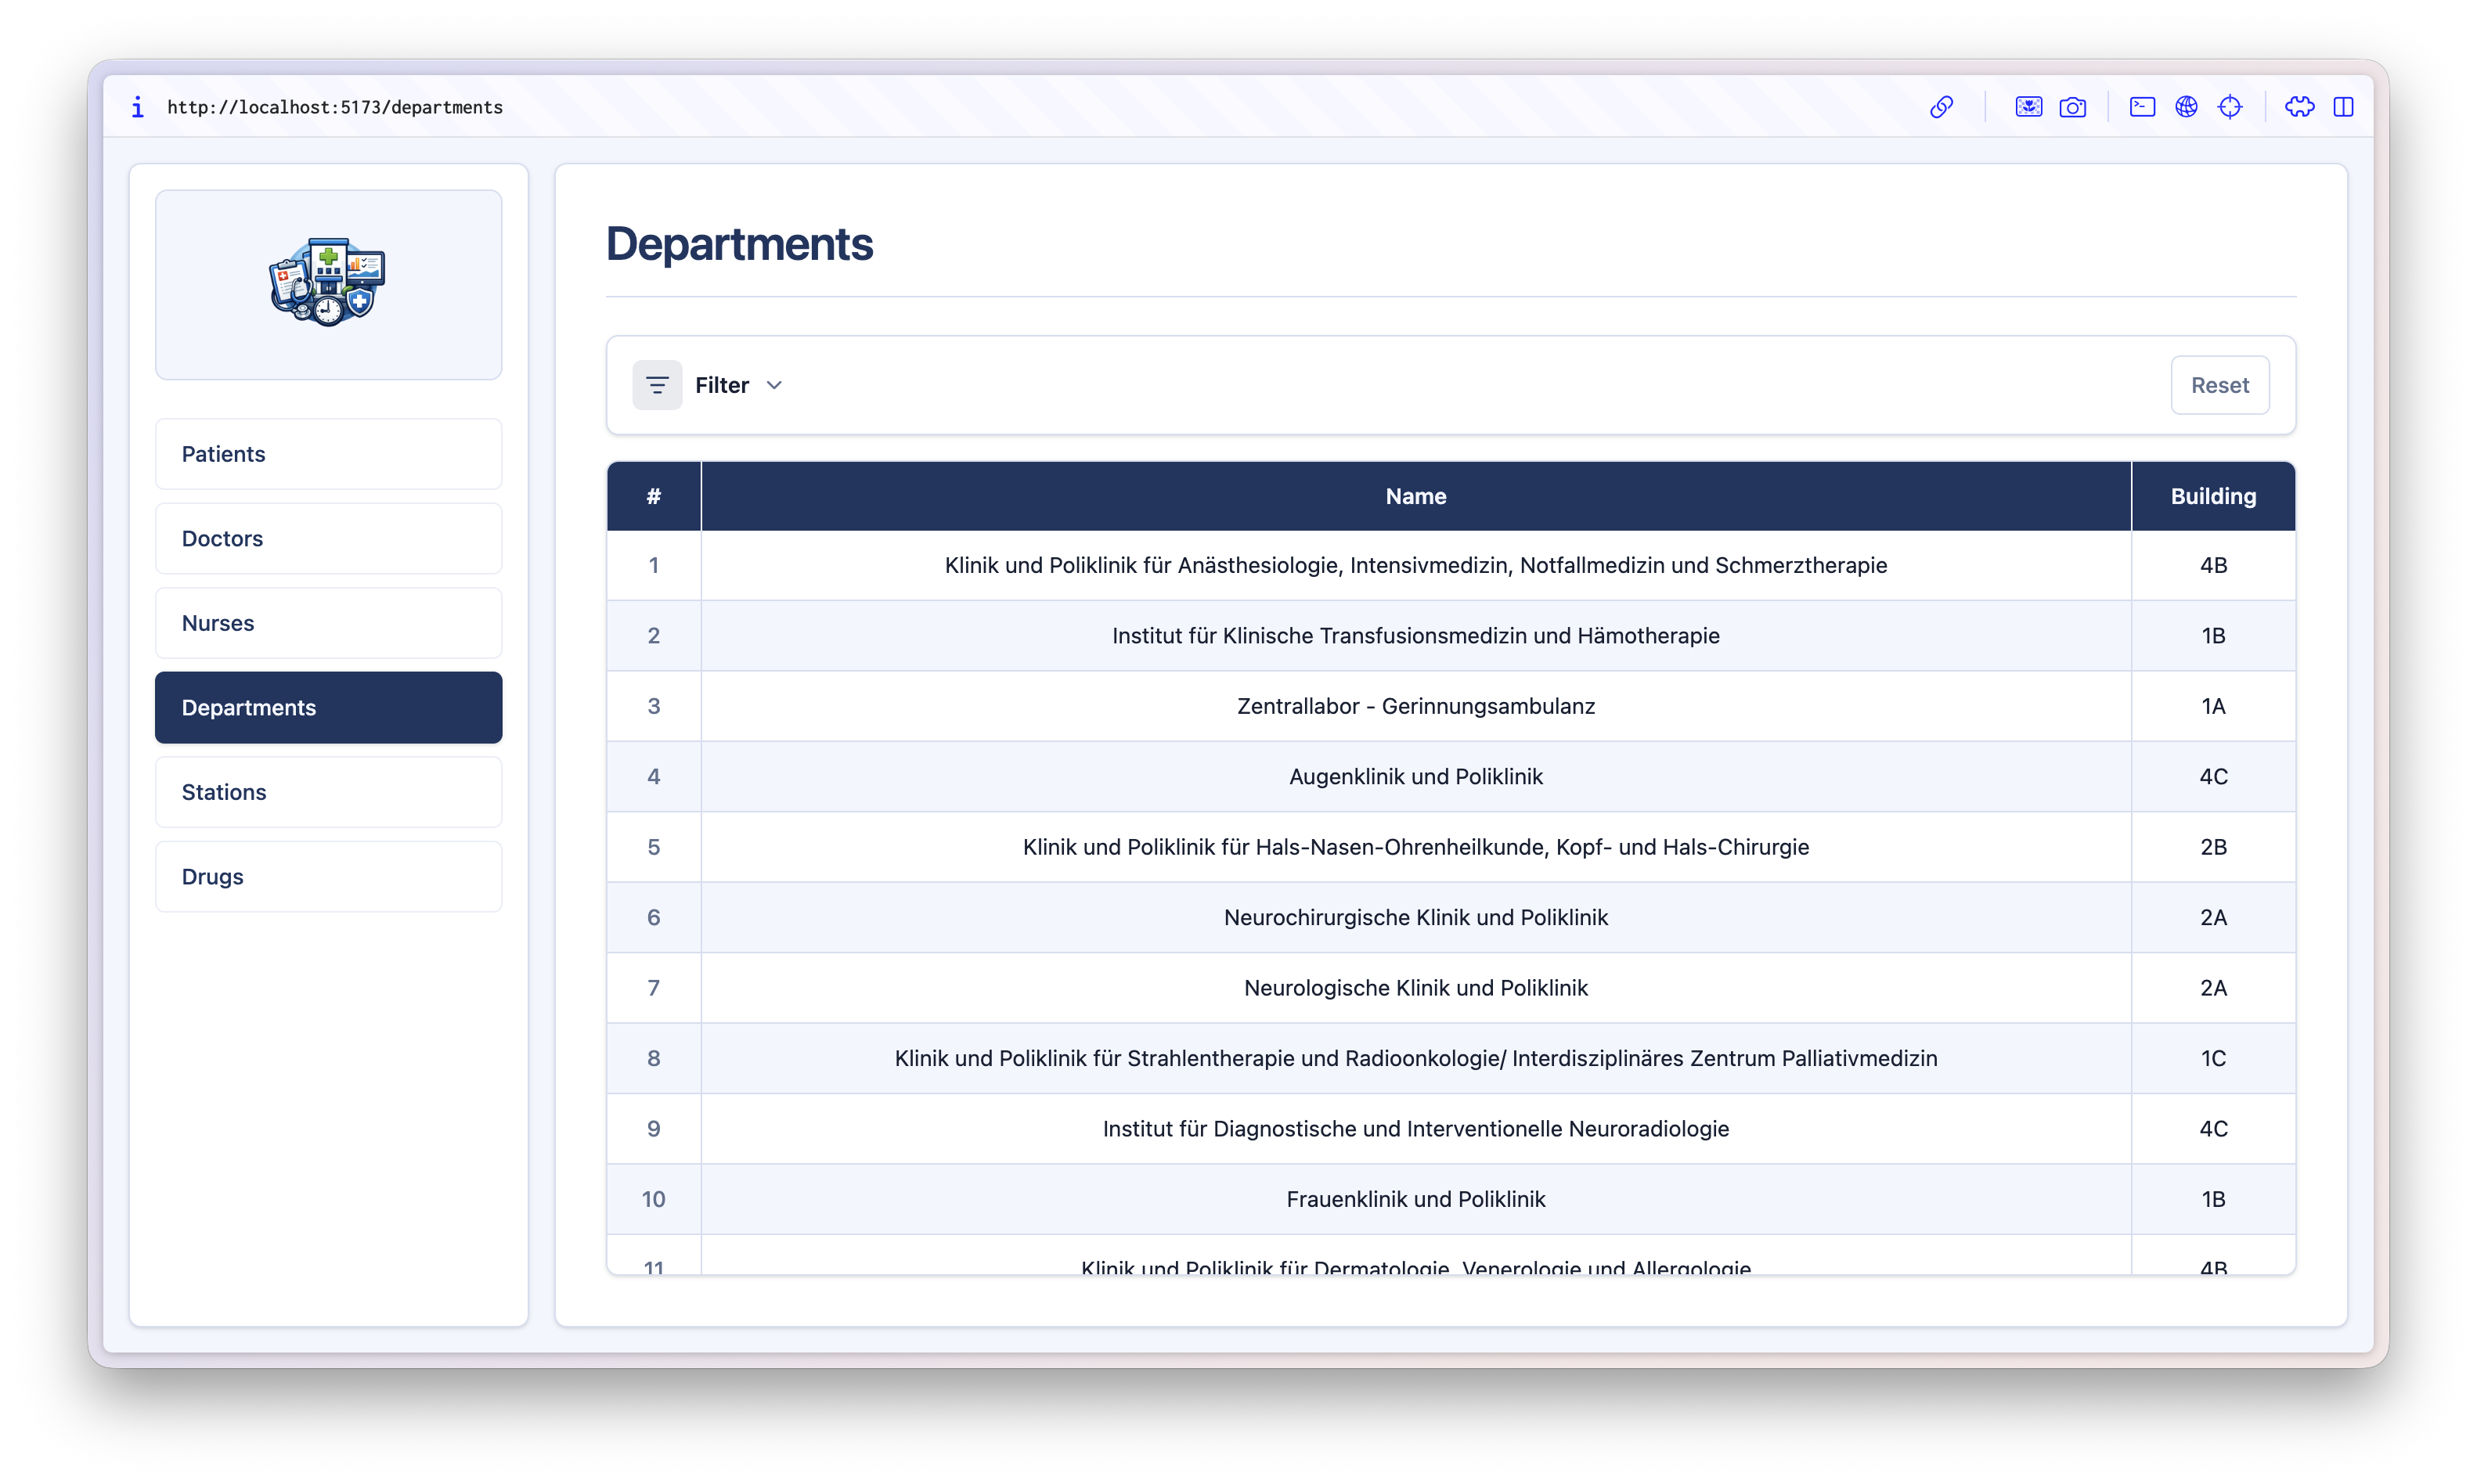
\includegraphics[width=\textwidth,height=0.78\textheight,keepaspectratio]{departments.png}
    \caption{Abteilungsübersicht}
    \label{fig:frontend-departments}
\end{figure}

\begin{figure}[H]
    \centering
    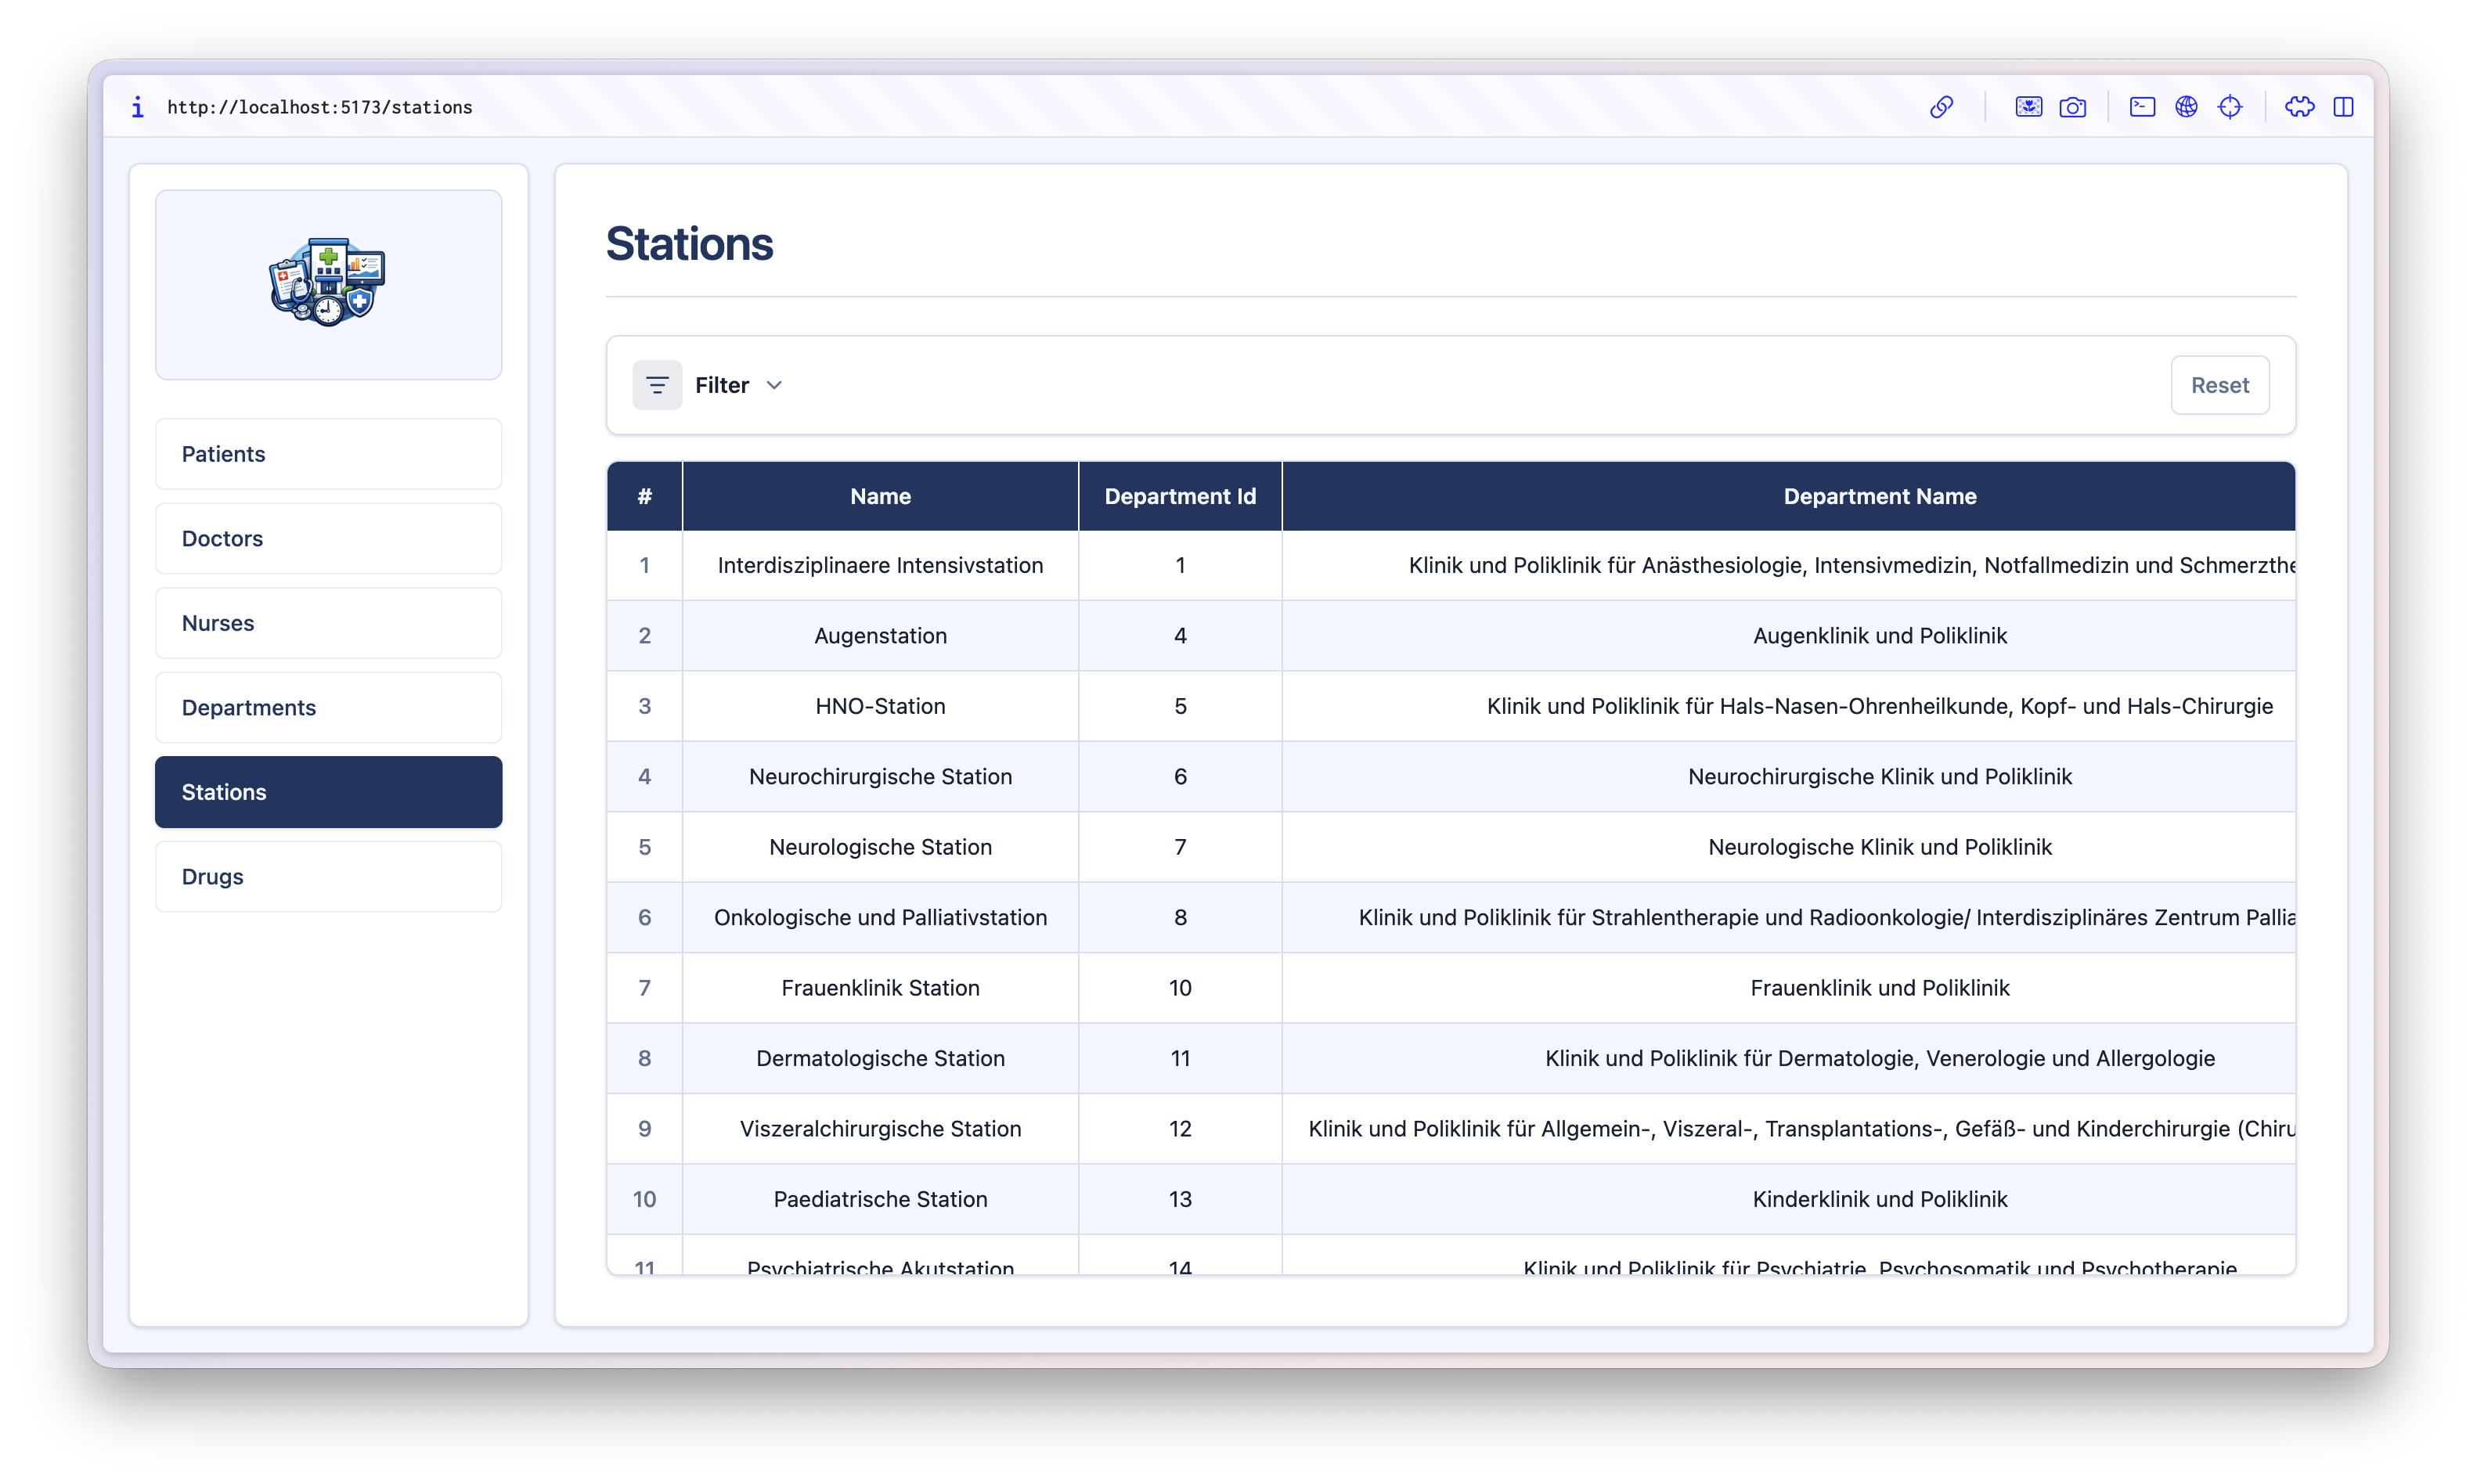
\includegraphics[width=\textwidth,height=0.78\textheight,keepaspectratio]{stations.png}
    \caption{Stationsübersicht}
    \label{fig:frontend-stations}
\end{figure}

\begin{figure}[H]
    \centering
    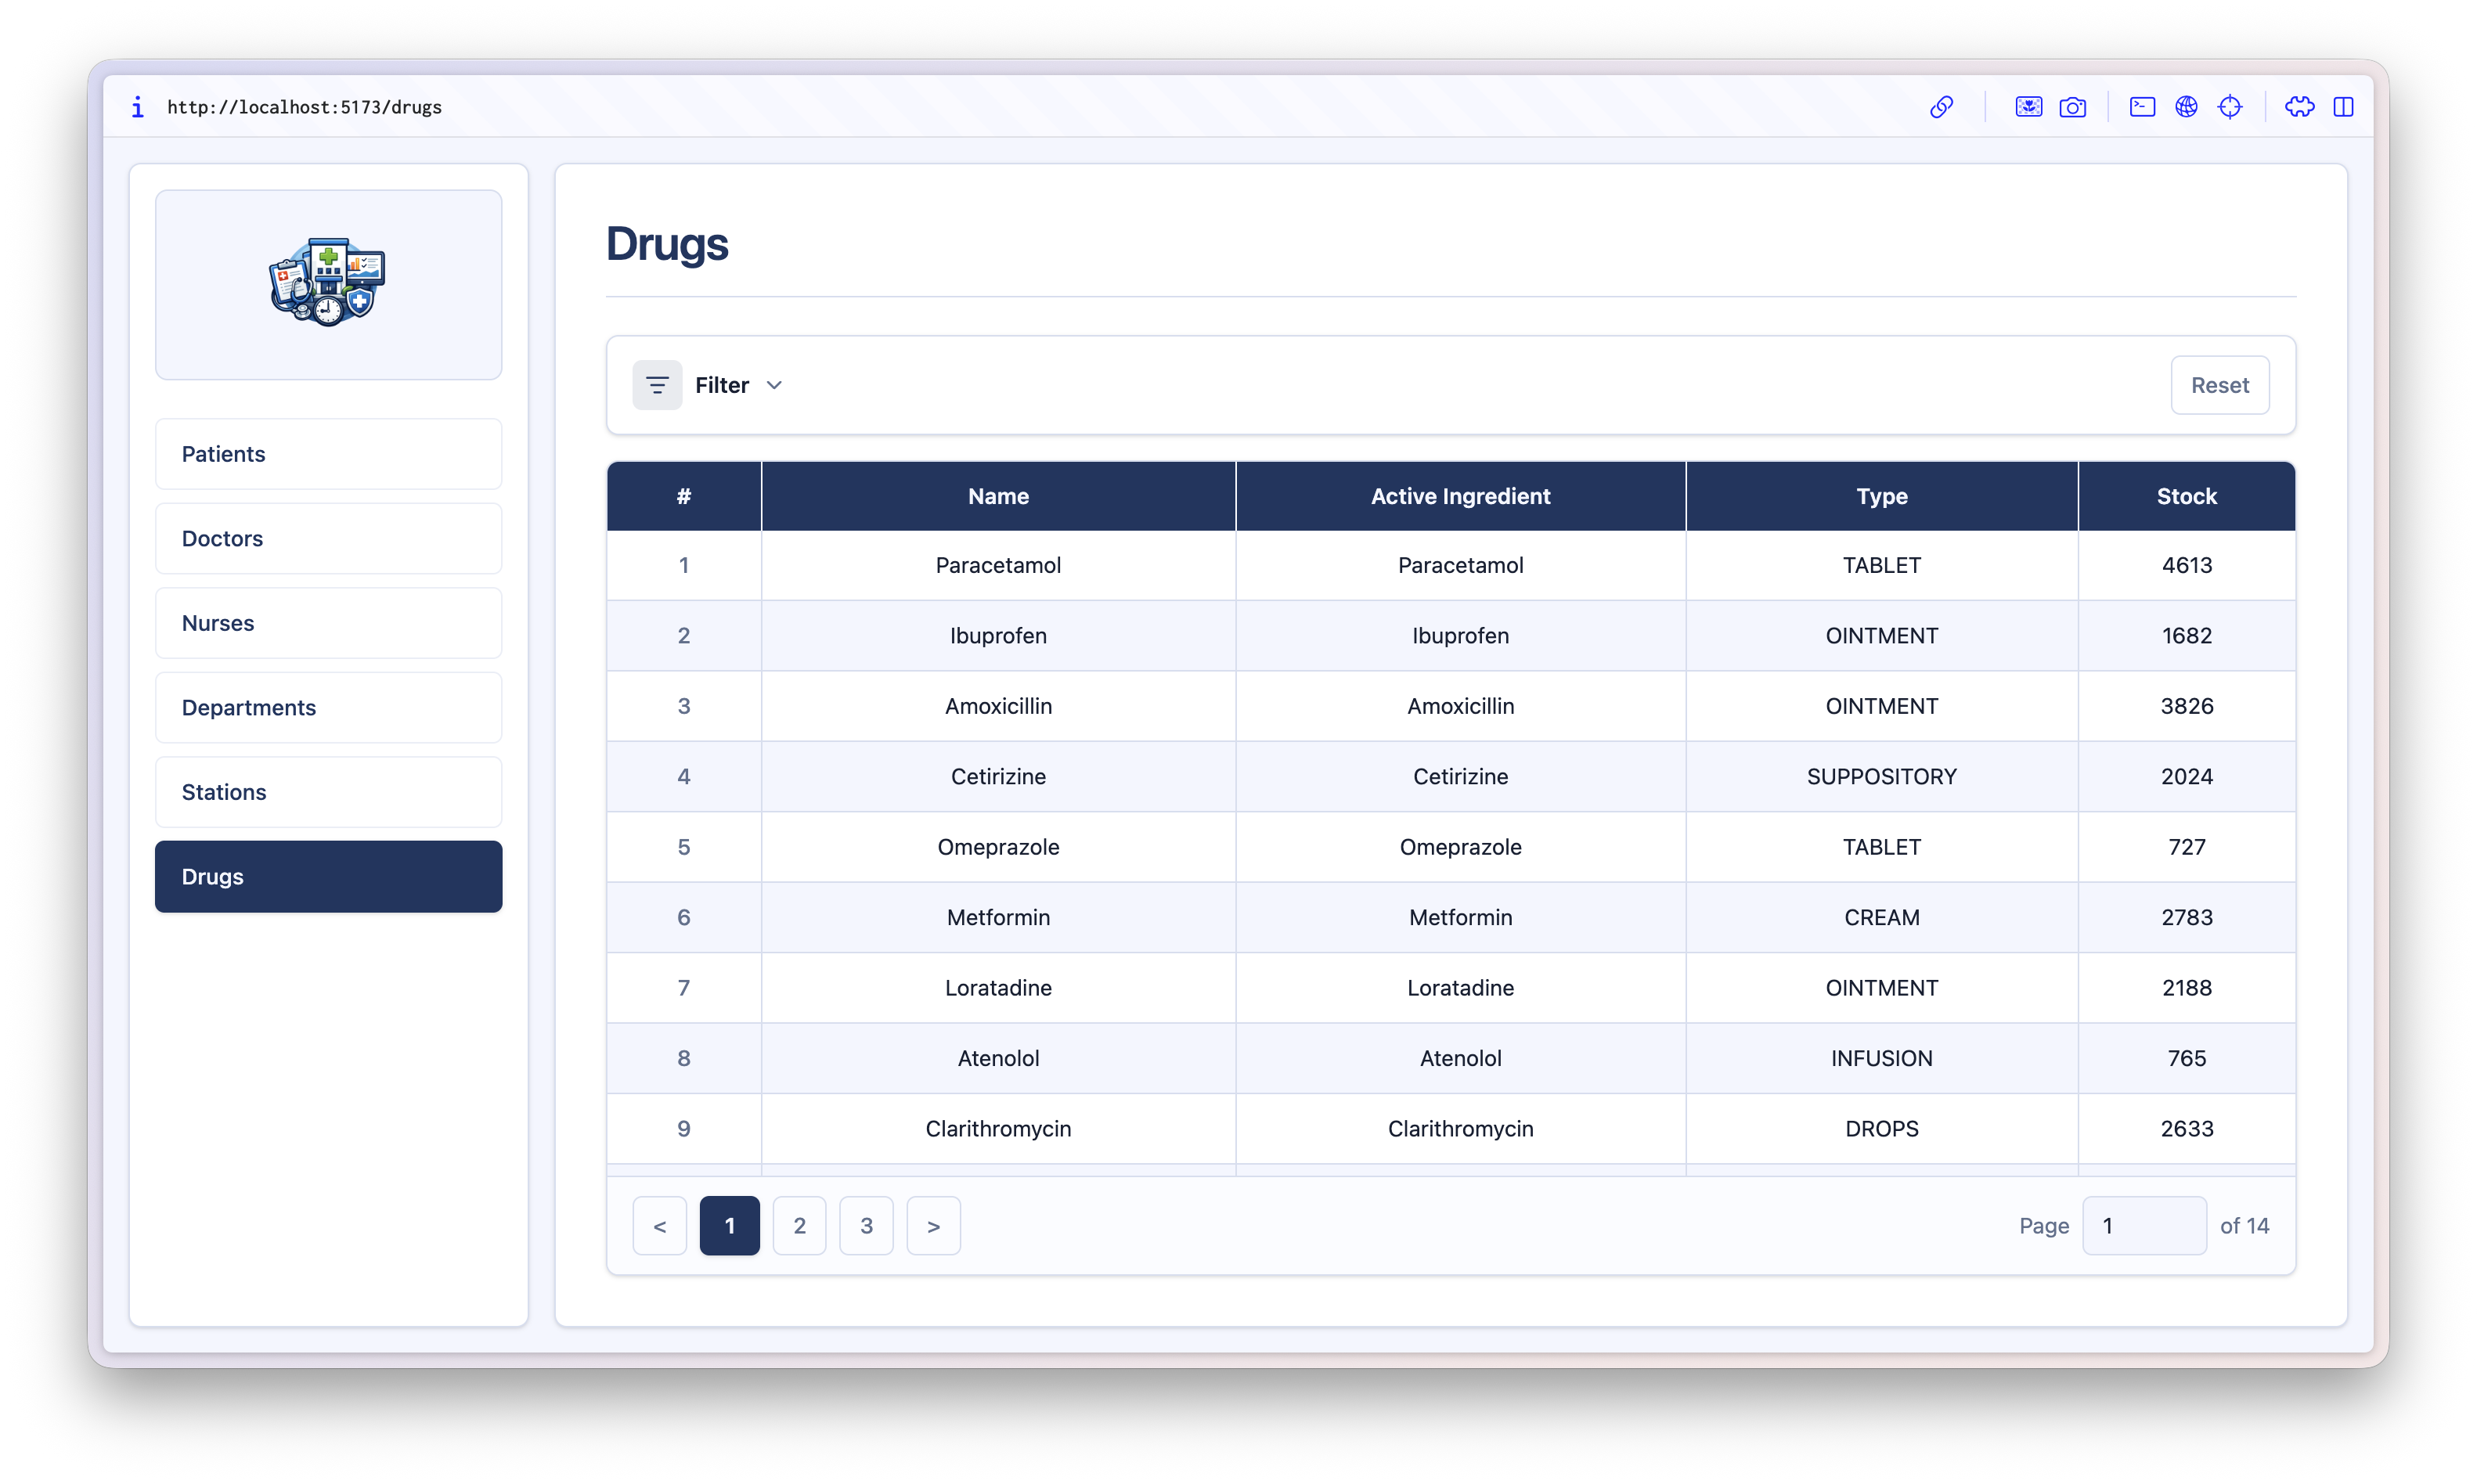
\includegraphics[width=\textwidth,height=0.78\textheight,keepaspectratio]{drugs.png}
    \caption{Medikamentenübersicht}
    \label{fig:frontend-drugs}
\end{figure}

\begin{figure}[H]
    \centering
    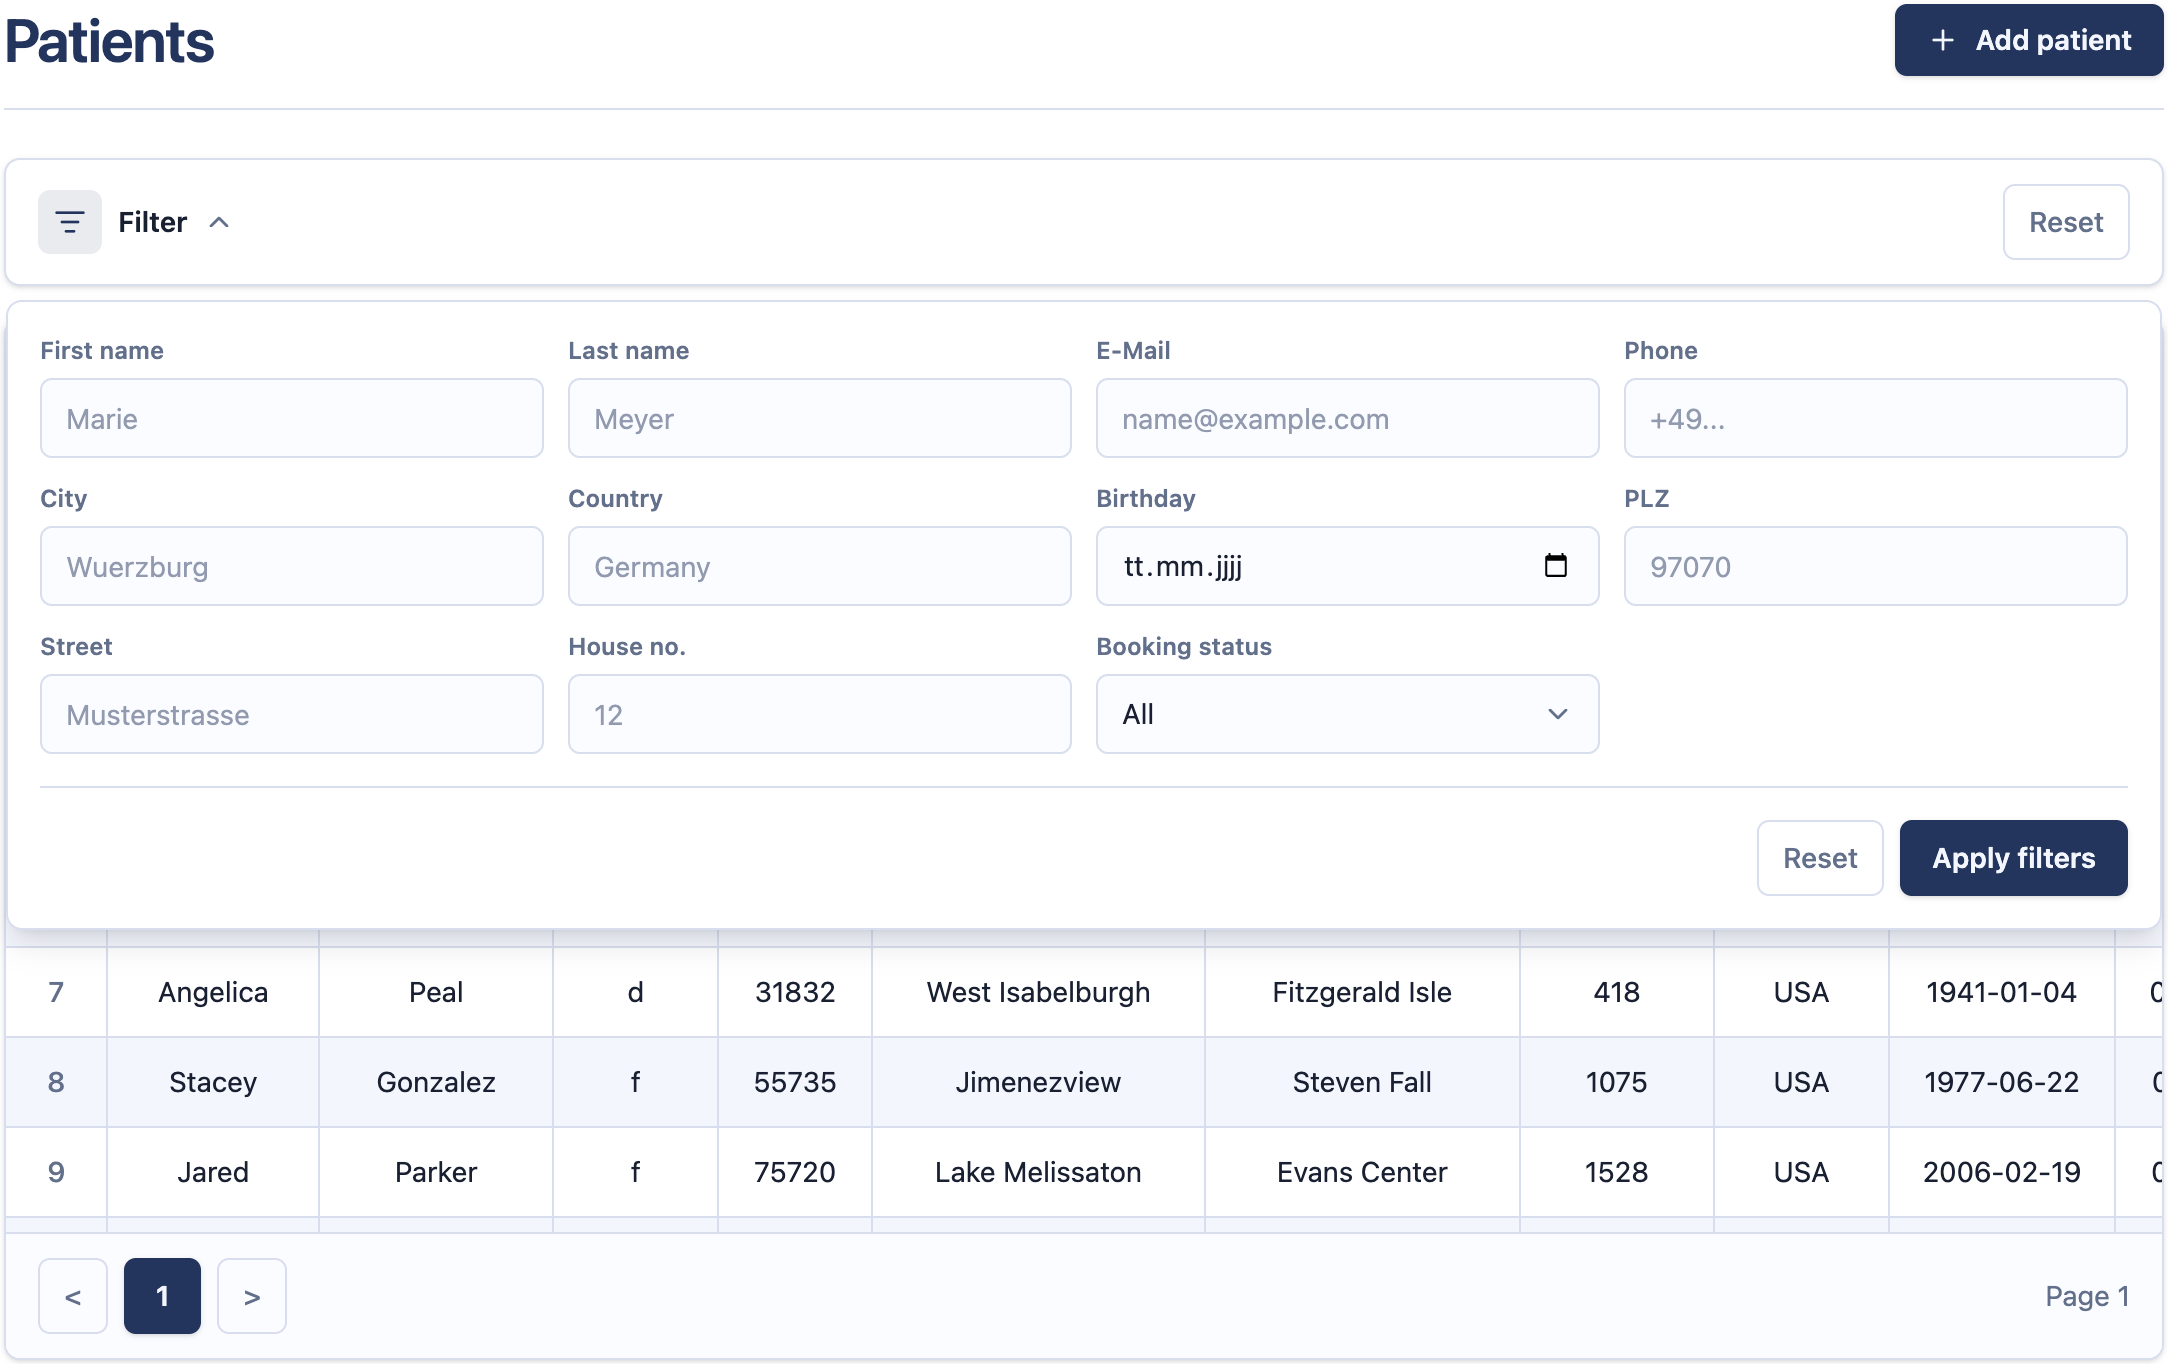
\includegraphics[width=\textwidth,height=0.78\textheight,keepaspectratio]{filter.png}
    \caption{Filterbereich der Tabellenansicht}
    \label{fig:frontend-filter}
\end{figure}

\subsection{Patientenaktionen}

\begin{figure}[H]
    \centering
    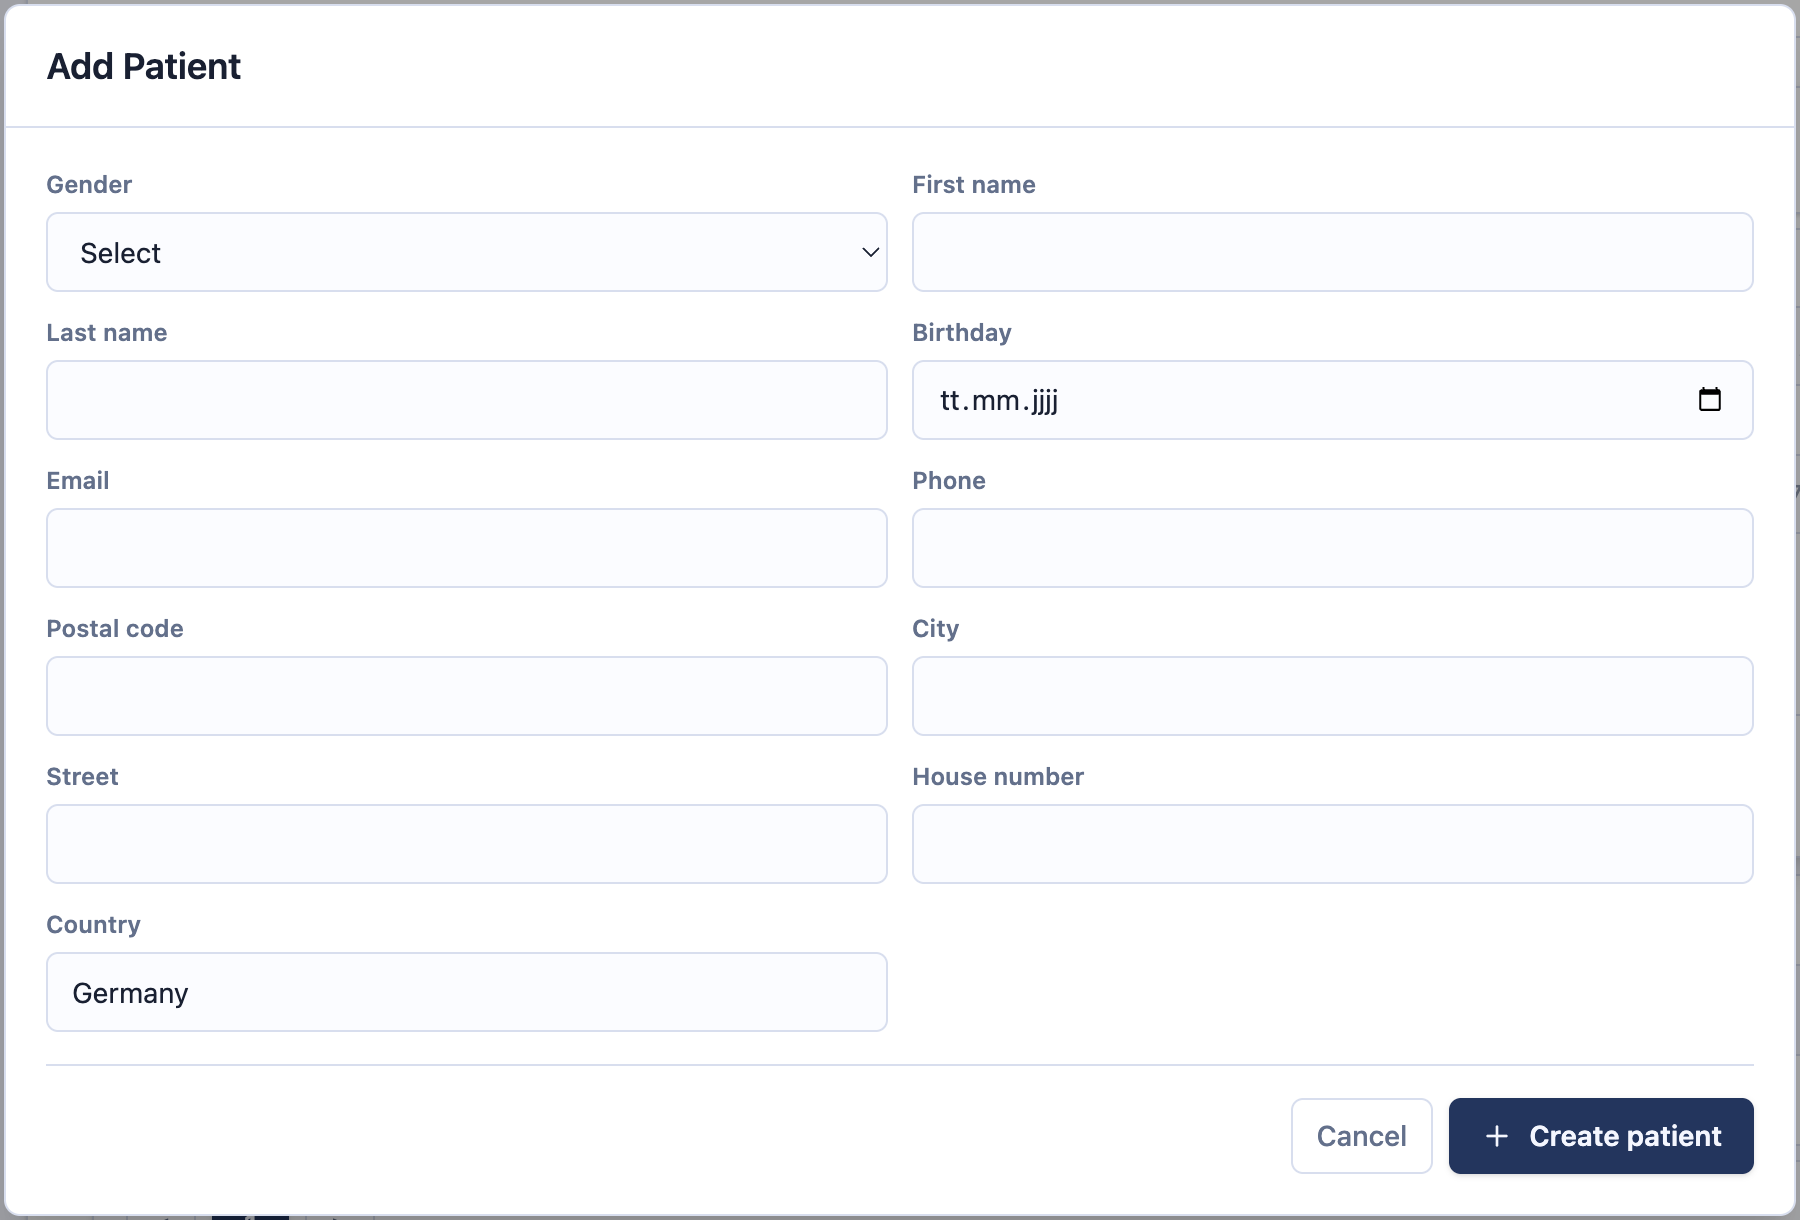
\includegraphics[width=\textwidth,height=0.78\textheight,keepaspectratio]{add-patient-modal.png}
    \caption{Dialog zum Anlegen eines Patienten}
    \label{fig:frontend-add-patient}
\end{figure}

\begin{figure}[H]
    \centering
    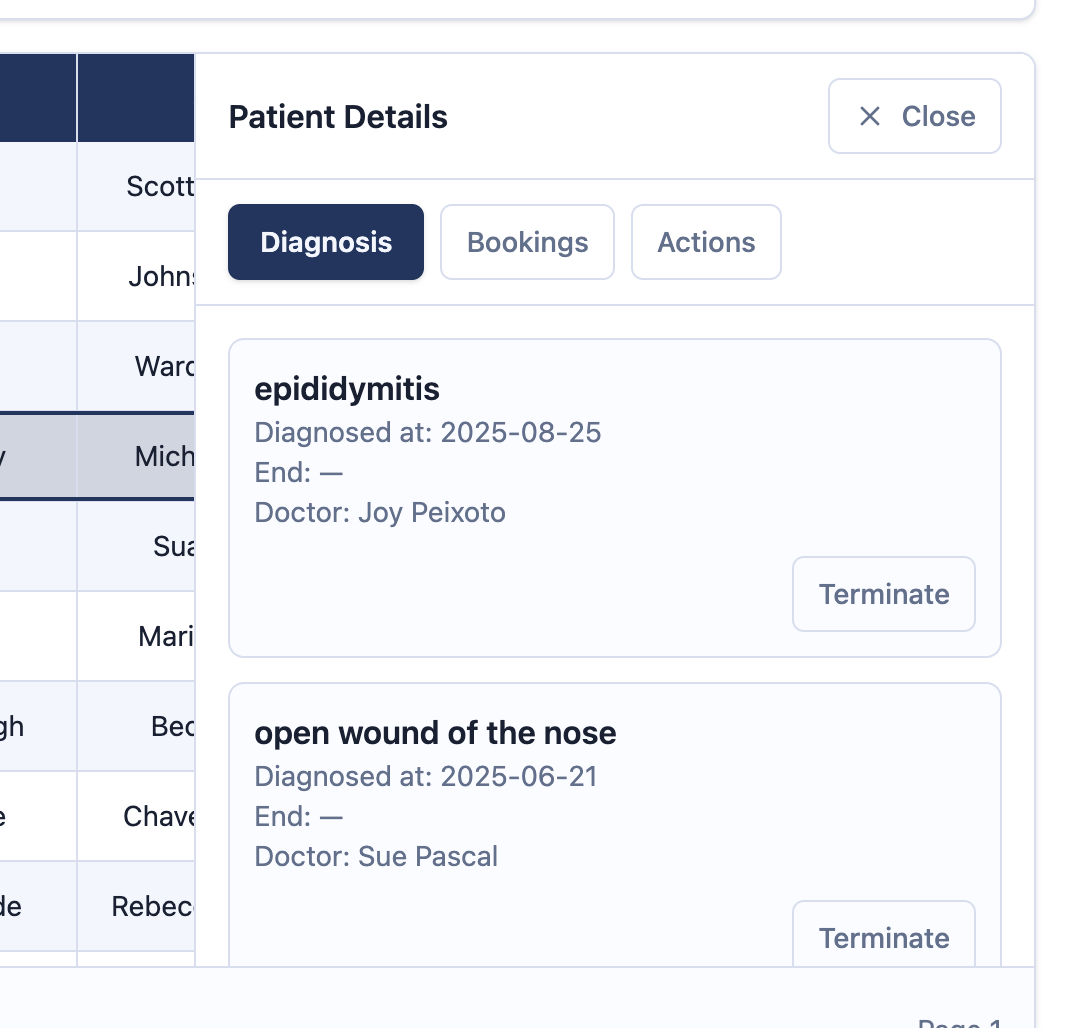
\includegraphics[width=\textwidth,height=0.78\textheight,keepaspectratio]{patient-details-diagnosis.png}
    \caption{Patientendetails mit Diagnosen}
    \label{fig:frontend-patient-diagnoses}
\end{figure}

\begin{figure}[H]
    \centering
    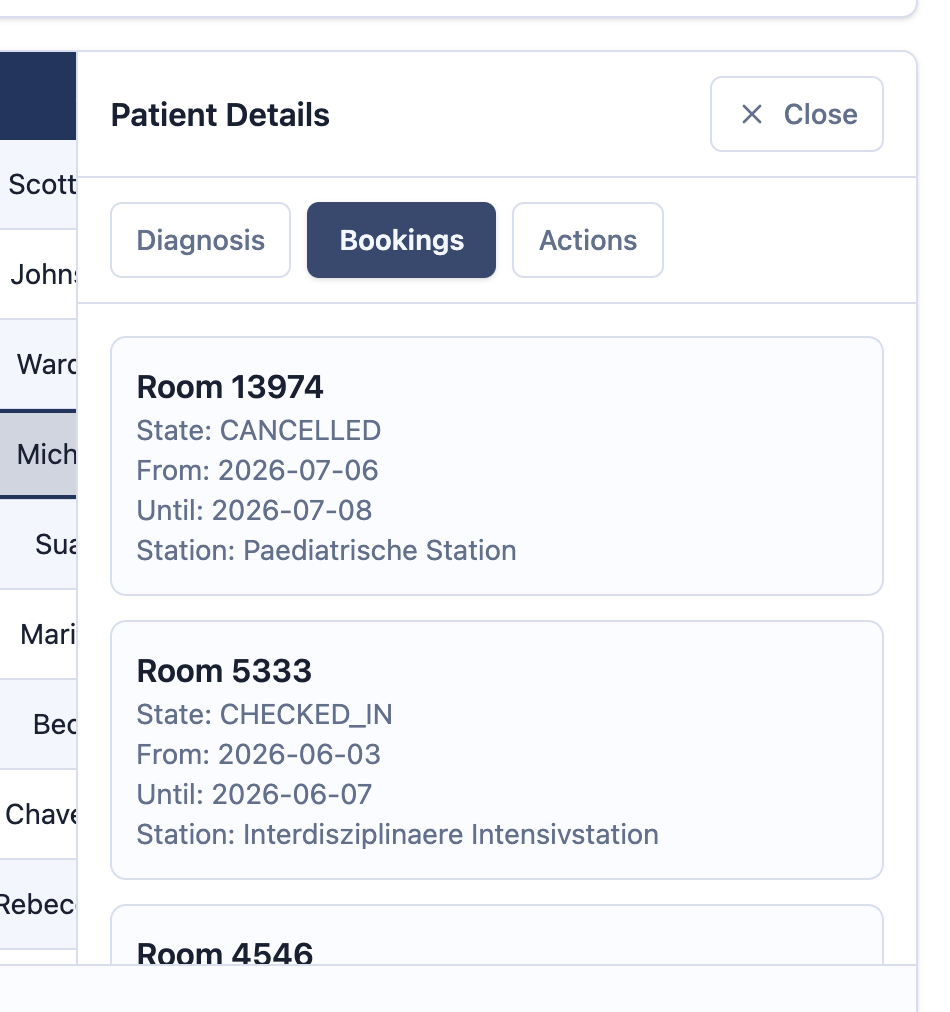
\includegraphics[width=\textwidth,height=0.78\textheight,keepaspectratio]{patient-details-bookings.png}
    \caption{Patientendetails mit Buchungen}
    \label{fig:frontend-patient-bookings}
\end{figure}

\begin{figure}[H]
    \centering
    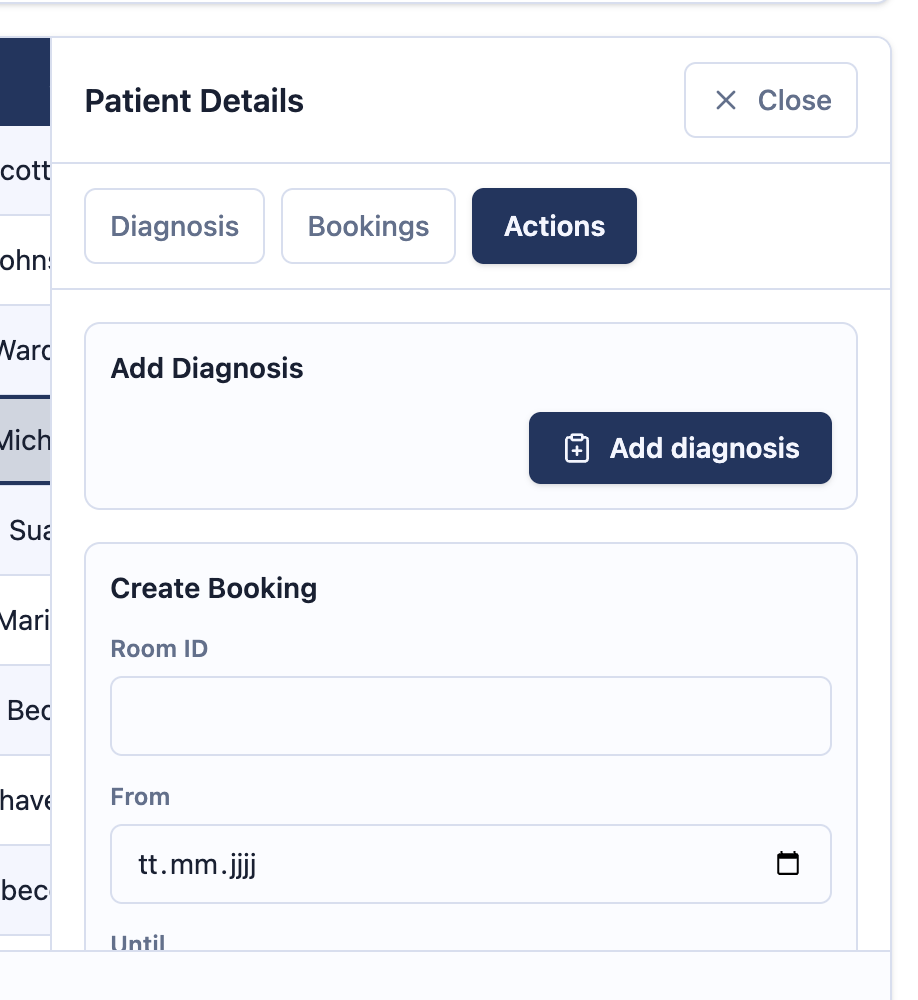
\includegraphics[width=\textwidth,height=0.78\textheight,keepaspectratio]{patient-details-actions-1.png}
    \caption{Patientenaktionen für Diagnose und Buchung}
    \label{fig:frontend-patient-actions-1}
\end{figure}

\begin{figure}[H]
    \centering
    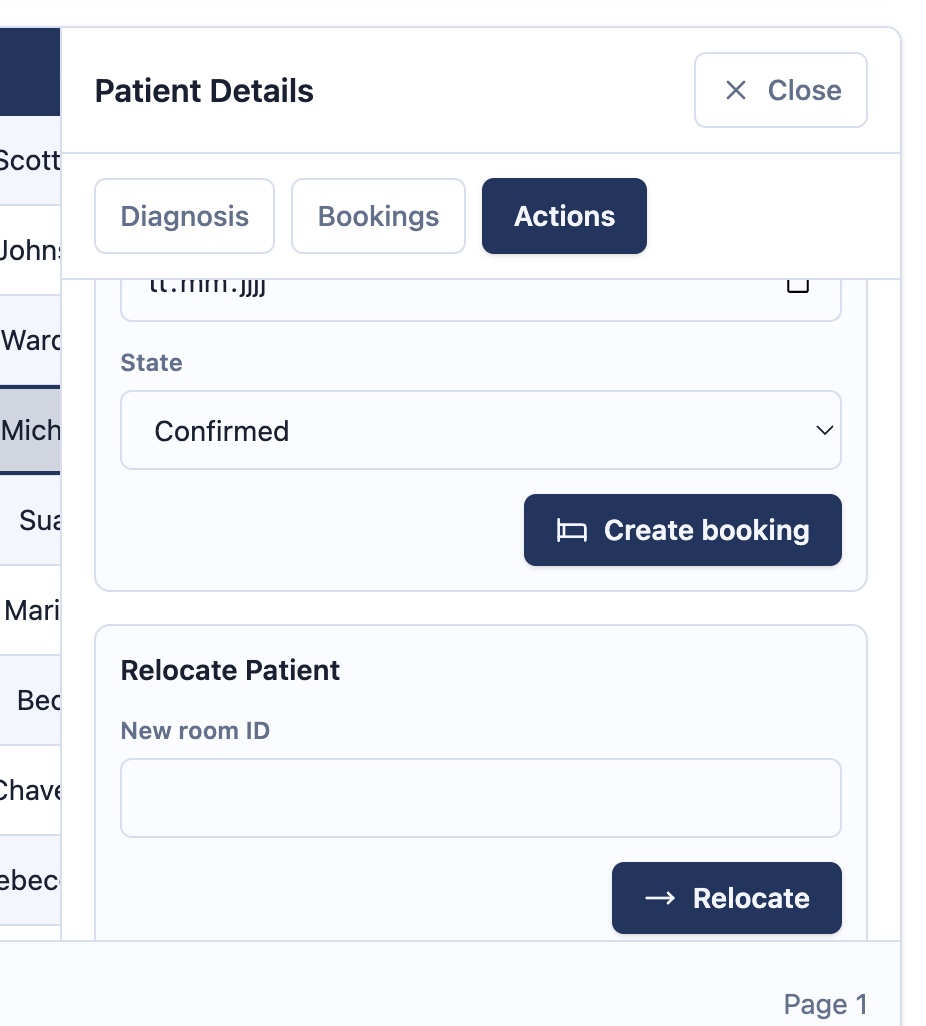
\includegraphics[width=\textwidth,height=0.78\textheight,keepaspectratio]{patient-details-actions-2.png}
    \caption{Patientenaktionen für Verlegung und Entlassung}
    \label{fig:frontend-patient-actions-2}
\end{figure}

\begin{figure}[H]
    \centering
    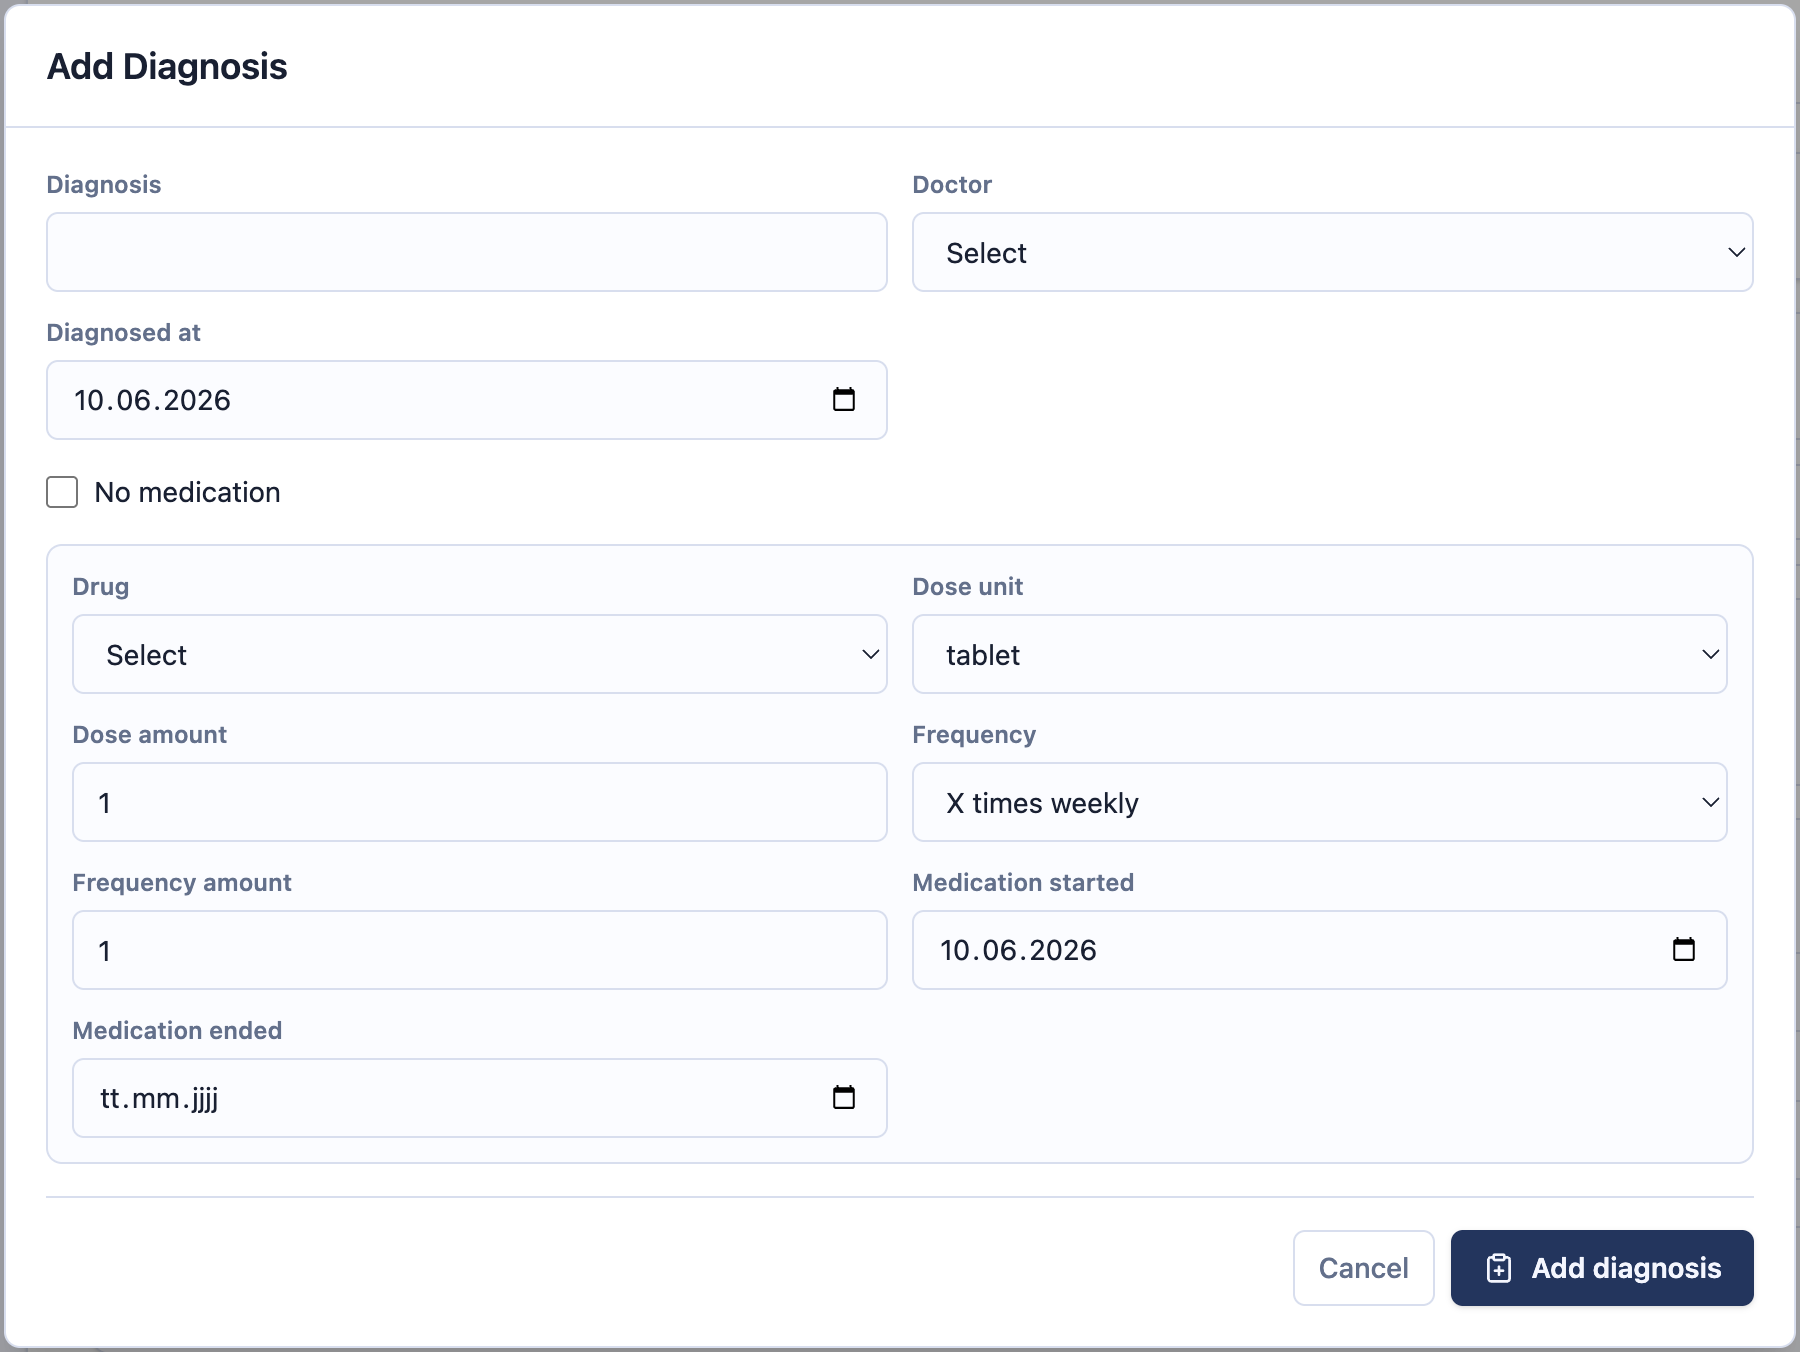
\includegraphics[width=\textwidth,height=0.78\textheight,keepaspectratio]{add-diagnosis-modal.png}
    \caption{Dialog zum Anlegen einer Diagnose mit Medikation}
    \label{fig:frontend-add-diagnosis}
\end{figure}
